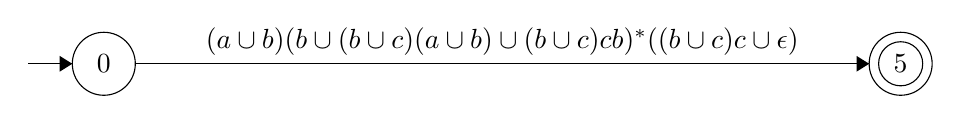
\begin{tikzpicture}[scale=0.2]
    \tikzstyle{every node}+=[inner sep=0pt]
    \draw [black] (5,-2.7) circle (2);
    \draw (5,-2.7) node {$0$};
    \draw [black] (55.6,-2.7) circle (2);
    \draw (55.6,-2.7) node {$5$};
    \draw [black] (55.6,-2.7) circle (1.4);
    \draw [black] (0.2,-2.7) -- (3,-2.7);
    \fill [black] (3,-2.7) -- (2.2,-2.2) -- (2.2,-3.2);
    \draw [black] (7,-2.7) -- (53.6,-2.7);
    \fill [black] (53.6,-2.7) -- (52.8,-2.2) -- (52.8,-3.2);
    \draw (30.3,-2.2) node [above] {$(a\cup b)(b\cup (b\cup c)(a\cup b)\cup (b\cup c)cb)^*((b\cup c)c\cup \epsilon)$};
    \end{tikzpicture}